% id: 74-21
% book: 쎈B 대수 · 06 삼각함수의 그래프
% section: 유형 06 삼각함수의 미정계수의 결정; 그래프가 주어진 경우
% figure: tikz:fig-74-21
% answer: 
% answer_source: 
% variant_level: 0 (원본 전사)
% 이 파일은 build.mjs 가 items.json 에서 만든다. 고칠 때는 items.json 을 고친다.
\smash{\raisebox{4.5mm}{\dmkichul{쎈B 대수 74쪽 21번}}}
\noindent\begin{minipage}[t]{0.58\linewidth}\vspace{0pt}\raggedright 함수 $y=a\sin \pi\left(x-\dfrac{1}{3}\right)+b$의 그래프가 오른쪽 그림과 같을 때, 상수 $a$, $b$, $c$에 대하여 $a+3b+6c$의 값은? \dmcondfill{$a>0$}{}\end{minipage}\hfill\begin{minipage}[t]{0.4\linewidth}\vspace{0pt}\centering \resizebox{\ifdim\width>\linewidth\linewidth\else\width\fi}{!}{% 74-21(74쪽) — $y=a\sin\pi\left(x-\frac{1}{3}\right)+b$ 의 그래프(최댓값 3 · 최솟값 $-1$ · 최댓값을 갖는 점 $\frac{5}{6}$ 과 최솟값을 갖는 점 $c$). 스캔 화질이 낮아 TikZ 로 다시 그림(원문 라벨·점선·화살표만).
\begin{tikzpicture}[line width=0.6pt, x=0.75cm, y=0.56cm, every node/.style={inner sep=1pt}]
  \draw[dotted, line width=0.5pt] (-1.0,3) -- (3.55,3);
  \draw[dotted, line width=0.5pt] (-1.0,-1) -- (3.55,-1);
  \draw[->, >=stealth, line width=0.7pt] (-1.1,0) -- (3.85,0) node[below=1pt] {$x$};
  \draw[->, >=stealth, line width=0.7pt] (0,-1.9) -- (0,3.9) node[left=1pt] {$y$};
  \draw[domain=-0.85:3.4, samples=160, smooth] plot (\x, {2*sin(180*(\x-0.33333))+1});
  \draw[dotted, line width=0.5pt] (0.83333,0) -- (0.83333,3);
  \draw[dotted, line width=0.5pt] (1.83333,0) -- (1.83333,-1);
  \node[anchor=south east, font=\small] at (-0.06,2.85) {$3$};
  \node[anchor=north east, font=\small] at (-0.06,-1.05) {$-1$};
  \node[anchor=north east, font=\small] at (0.0,-0.03) {$\pt{O}$};
  \node[anchor=south, font=\small] at (1.76,0.08) {$c$};
  \node[font=\small] (fiveosix) at (1.35,-1.6) {$\dfrac{5}{6}$};
  \draw[->, >=stealth, line width=0.4pt] (fiveosix.north) to[bend right=25] (0.92,-0.15);
  \node[anchor=south west, font=\small] at (0.3,3.05) {$y=a\sin \pi\left(x-\dfrac{1}{3}\right)+b$};
\end{tikzpicture}
}\end{minipage}\par
\dmchoicesauto{}{$8$}{$10$}{$12$}{$14$}{$16$}
